\documentclass[a4 paper]{article}

% Set target color model to RGB
\usepackage[inner=2.0cm,outer=2.0cm,top=2.5cm,bottom=2.5cm]{geometry}
\usepackage{setspace}
\usepackage[rgb]{xcolor}
\usepackage{verbatim}
\usepackage{subcaption}
\usepackage{amsgen,amsmath,amstext,amsbsy,amsopn,tikz,amssymb,tkz-linknodes}
\usepackage{fancyhdr}
\usepackage[colorlinks=true, urlcolor=blue,  linkcolor=blue, citecolor=blue]{hyperref}
\usepackage[colorinlistoftodos]{todonotes}
\usepackage{rotating}
%\usetikzlibrary{through,backgrounds}
\hypersetup{%
pdfauthor={Nabeel Warsalee},%
pdftitle={COMP3005 Final Project Report},%
pdfkeywords={Tikz,latex,bootstrap,uncertaintes},%
pdfcreator={PDFLaTeX},%
pdfproducer={PDFLaTeX},%
}
%\usetikzlibrary{shadows}
% \usepackage[francais]{babel}
\usepackage{booktabs}
\newcommand{\ra}[1]{\renewcommand{\arraystretch}{#1}}

\newtheorem{thm}{Theorem}[section]
\newtheorem{prop}[thm]{Proposition}
\newtheorem{lem}[thm]{Lemma}
\newtheorem{cor}[thm]{Corollary}
\newtheorem{defn}[thm]{Definition}
\newtheorem{rem}[thm]{Remark}
\numberwithin{equation}{section}

\newcommand{\homework}[6]{
   \pagestyle{myheadings}
   \thispagestyle{plain}
   \newpage
   \setcounter{page}{1}
   \noindent
   \begin{center}
   \framebox{
      \vbox{\vspace{2mm}
    \hbox to 6.28in { {\bf COMP 3005:~Database Management Systems \hfill {\small (#2)}} }
       \vspace{6mm}
       \hbox to 6.28in { {\Large \hfill #1  \hfill} }
       \vspace{6mm}
       \hbox to 6.28in { {\it Instructor: {\rm #3} \hfill Name: {\rm #5}, ID: {\rm #6}} }
       %\hbox to 6.28in { {\it TA: #4  \hfill #6}}
      \vspace{2mm}}
   }
   \end{center}
   \markboth{#5 -- #1}{#5 -- #1}
   \vspace*{4mm}
}

\newcommand{\problem}[2]{~\\\fbox{\textbf{Q #1}}\hfill (#2 points)\newline\newline}
\newcommand{\subproblem}[1]{~\newline\textbf{(#1)}}
\newcommand{\D}{\mathcal{D}}
\newcommand{\Hy}{\mathcal{H}}
\newcommand{\VS}{\textrm{VS}}
\newcommand{\solution}{~\newline\textbf{\textit{(Solution)}} }

\newcommand{\bbF}{\mathbb{F}}
\newcommand{\bbX}{\mathbb{X}}
\newcommand{\bI}{\mathbf{I}}
\newcommand{\bX}{\mathbf{X}}
\newcommand{\bY}{\mathbf{Y}}
\newcommand{\bepsilon}{\boldsymbol{\epsilon}}
\newcommand{\balpha}{\boldsymbol{\alpha}}
\newcommand{\bbeta}{\boldsymbol{\beta}}
\newcommand{\0}{\mathbf{0}}


\begin{document}
\homework{COMP3005 Final Project Report}{Due: Dec. 10th, 2021 (11:59 PM)}{Ahmed El-Roby}{}{}{}

\section*{Introduction}
This is the project report for the COMP3005A Final Project for the Fall 2021 term.\\
The group for this project consists of the following members...\\

\noindent\underline{\textbf{Group Members}}
\begin{itemize}
	\item Aaron Buitenwerf ()
	\item Hadi Cheaito ()
	\item Nabeel Warsalee (101103167)
\end{itemize}

\noindent All project files and source code can be found at the following \href{https://github.com/COMP3005A-Project/bookstore}{Github repository}...

\section{Conceptual Design}
Insert preamble about design.\\

\noindent\underline{\textbf{Assumptions Made}}\\
In this section we list all the assumptions that were made for certain aspects of the problem statement. These assumptions reflect how we designed and organized our database for this project.

\begin{itemize}
	\item A book can only have one publisher
	\item All books with same title have the same ISBN
	\item Assume an order can only have one of the same book (i.e., user cannot buy two copies of the same book)
	\item Each publisher has only one bank account
	\item There is only one report made per publisher
\end{itemize}

\noindent\underline{\textbf{ER Diagram}}\\
The following is the Entity-Relationship Diagram created to model the entities and relationships from the provided problem statement using the assumptions we have outlined above.\\

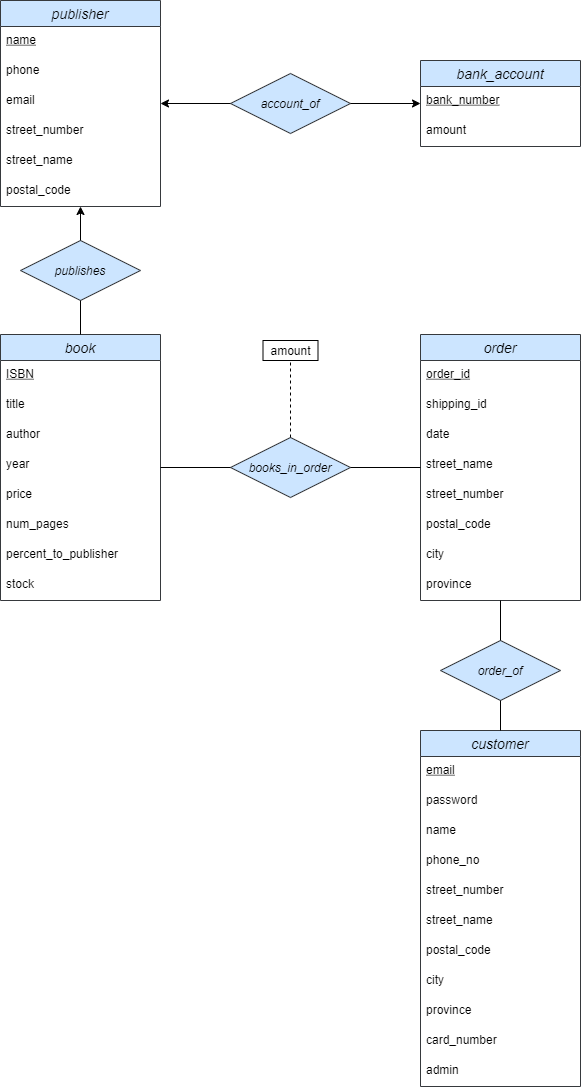
\includegraphics[scale=0.5]{../Diagrams/ER-diagram-bookstore-comp3005-finalproject.drawio.png}\\

\section{Reduction to Relation Schemas}
Here are the relation schemas gained from reducing our ER diagram into relations... (Note: Primary keys are underlined)\\

book(\underline{ISBN}, publisher\_name, stock, title, author, year, price, num\_pages, percent\_to\_publisher)\\
\indent order(\underline{order\_id}, email, shipping\_id, date, street\_number, street\_name, postal\_code, city, province)\\
\indent books\_in\_order(\underline{order\_id}, \underline{ISBN}, amount)\\
\indent customer(\underline{email}, password, name, phone, street\_number, street\_name, postal\_code, city, province, card\_number)\\
\indent publisher(\underline{name}, phone, bank\_number, email, street\_number, street\_name, postal\_code)\\
\indent bank\_account(\underline{bank\_number}, amount)\\

\section{Normalization of Relation Schemas}

\section{Database Schema Diagram}

The following is the Schema Diagram created to model schemas gained from our ER diagram and after normalization.\\

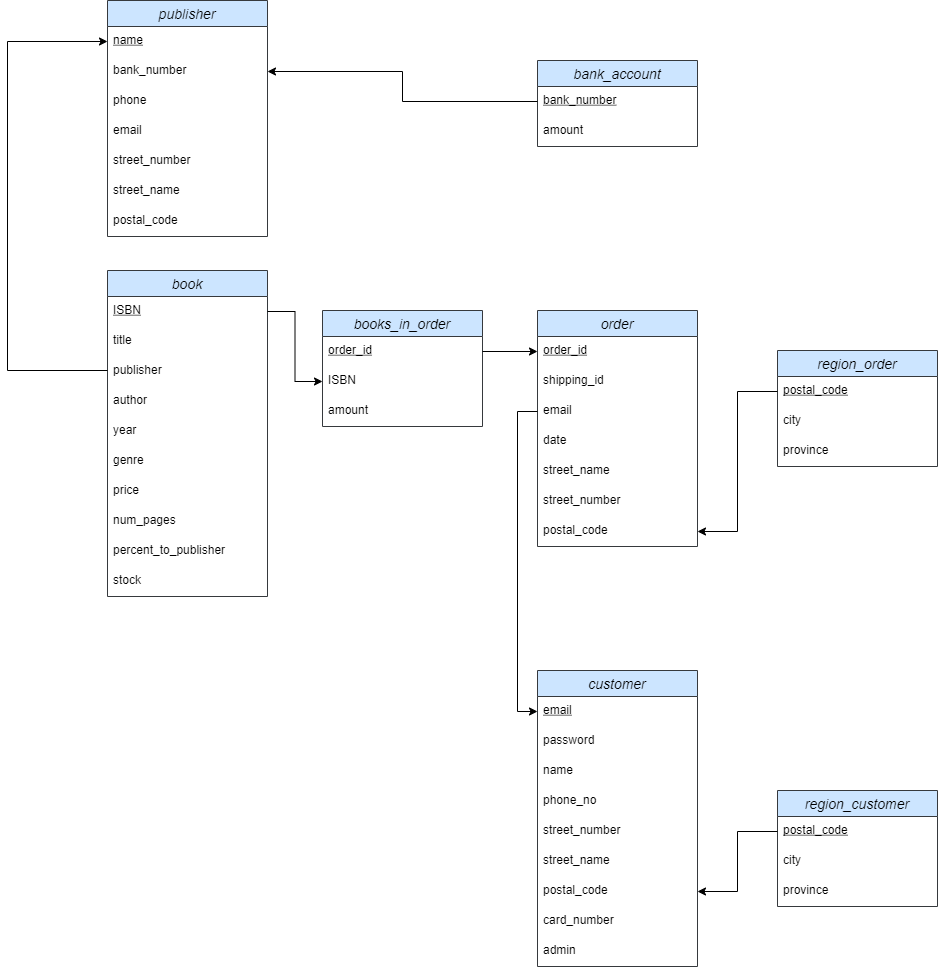
\includegraphics[scale=0.5]{../Diagrams/Schema-diagram-comp3005-finalproject.drawio.png}\\

\end{document}